Afin de réaliser notre station météo mobile, nous avons deux montages à
réaliser :
\begin{itemize}
\item le serveur (Raspberry Pi)
\item la station mobile (Arduino motorisée)
\end{itemize}

\section{Serveur}
Le serveur n'a besoin que d'un émetteur/récepteur radio nRF24l01 pour
fonctionner. De plus, il est nécessaire d'être connecté à internet pour être
accessible de l'extérieur.

\begin{center}
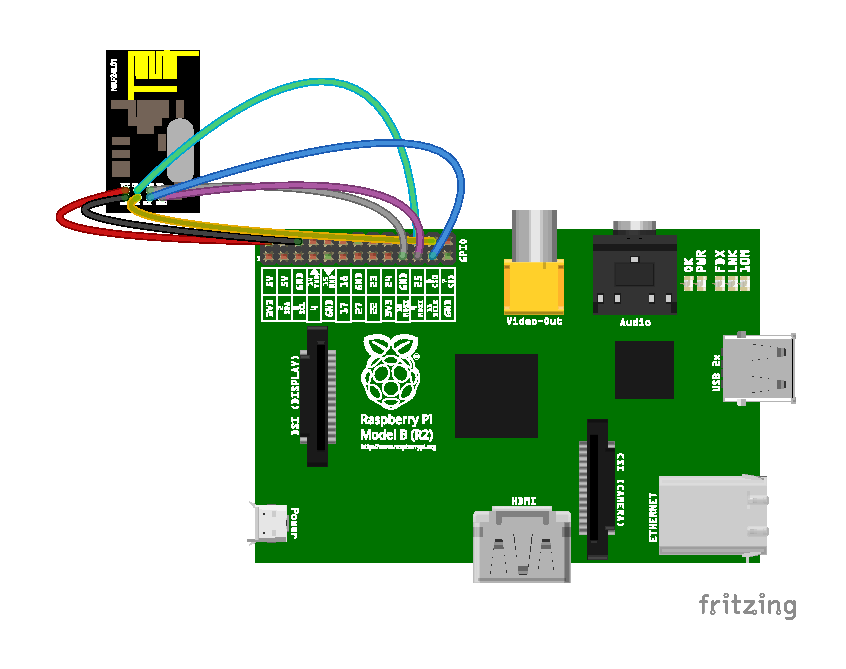
\includegraphics[scale=1]{include/raspberry_bb.pdf}
\end{center}


\textbf{Code couleur du cablage du nRF24l01}\\
\begin{center}
\begin{tabular}{l|c}
Couleur & Broche \\
\hline
Jaune  & CE\\
Vert   & CS\\
Bleu   & SCK\\
Violet & MISO\\
Gris   & MOSI\\
Rouge  & VCC\\
Noir   & GND
\end{tabular}
\end{center}
\pagebreak
\section{Station mobile}
Pour la réalisation de la partie mobile, nous aurons besoin :
\begin{itemize}
\item d'un Arduino (Mega dans notre cas),
\item de 2 moteurs (des servos-moteurs ici, mais vous pouvez utiliser d'autres
types de motorisations, comme un moteur de propulsion et un servo-moteur de 
direction par exemple),
\item une thermistance,
\item une résistance de 220$\Omega$,
\item un capteur de température,
\item un nRF24l01,
\item une alimentation 5V (des piles dans notre cas)
\end{itemize}

\paragraph{}
Le montage sera le suivant :
\begin{center}
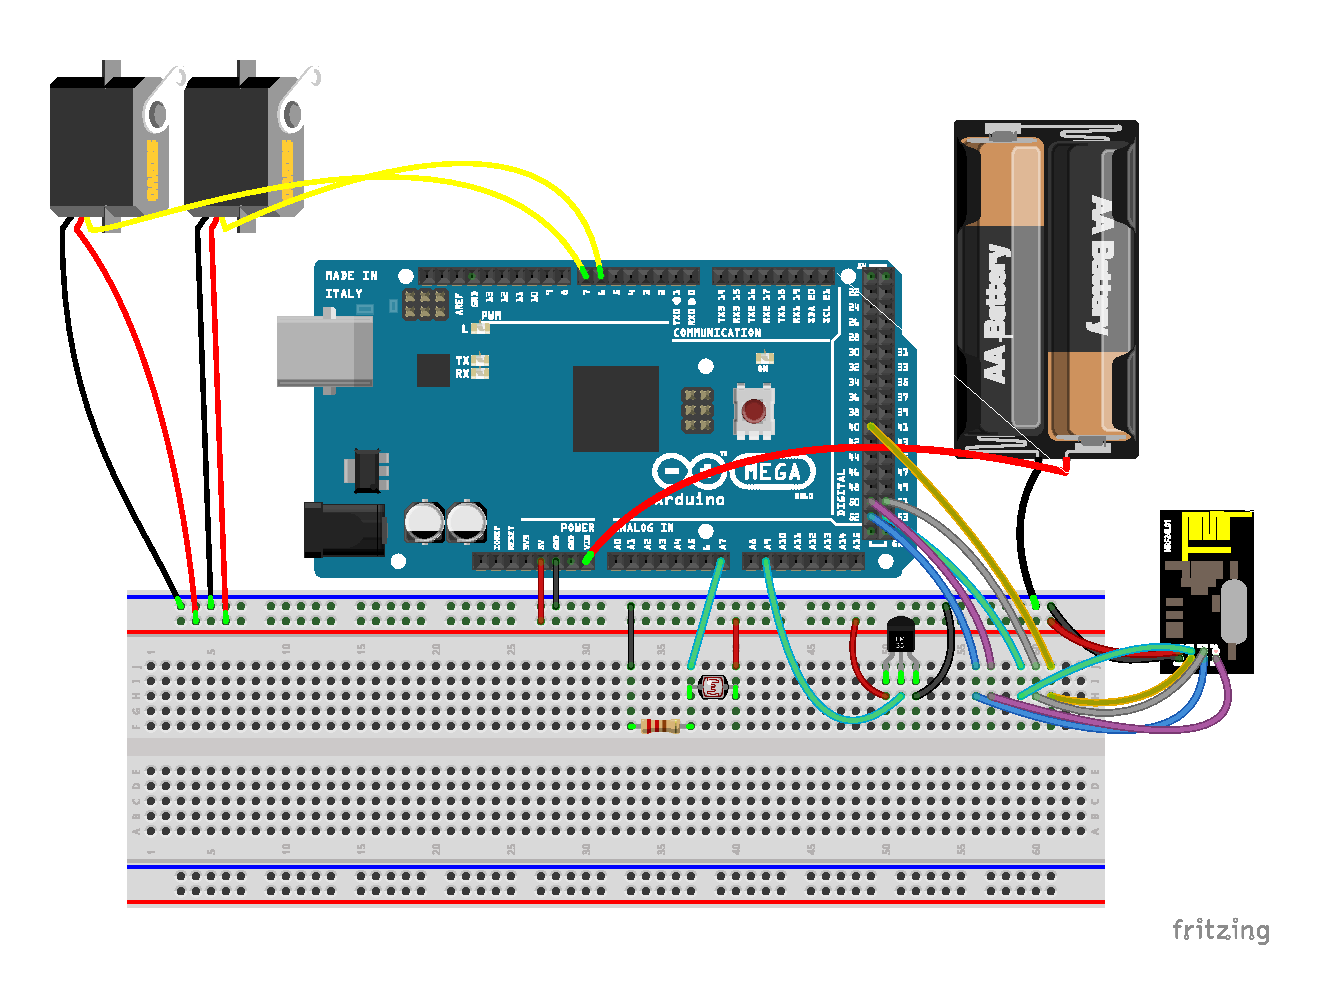
\includegraphics[scale=0.7]{include/arduino_bb.pdf}
\end{center}

\paragraph{}
Le code couleur pour la connectique du nRF24l01 est la même que précédemment
pour la Raspberry. De plus, on ne parlera pas ici de l'aspect mécanique 
(chassis, placement des moteurs, etc...).
